\documentclass{beamer}
\usepackage{amsmath,amssymb,latexsym,array,fancyheadings,mathdots}
\usepackage{algorithm,algorithmic}
\usepackage{hyperref}
\usepackage{color}
\usepackage{tabularx}
\usepackage[all]{xy}
\usepackage{qtree}
\usepackage{gitinfo2}

%% RCS
%\usepackage{rcs}

%% Colors
\definecolor{darkgreen}{rgb}{0,.4,0}
\definecolor{darkred}{rgb}{.5,0,0}
\definecolor{darkmagenta}{rgb}{.5,0,.5}
\definecolor{orange}{rgb}{1,.5,0}
\definecolor{lightblue}{rgb}{0.122,0.016,0.855}
\definecolor{darkocre}{rgb}{0.471,0.298,0.008}

\usetheme{default}

%% New Theorems
\newtheorem{thm}{Theorem}
\newtheorem{exm}[thm]{Example}
\newtheorem{cor}[thm]{Corollary}
\newtheorem{propo}[thm]{Proposition}
\newtheorem{lem}[thm]{Lemma}
\newtheorem{clm}[thm]{Claim}
\newtheorem{exr}[thm]{Exercise}
\newtheorem{dfn}[thm]{Definition}

%% New commands
\newcommand{\classfont}{\mathsf}
\newcommand{\ATM}{\classfont{A}_{\mathrm{TM}}}
\newcommand{\MTF}{\mathrm{MTF}}
\newcommand{\OPT}{\mathrm{OPT}}
\newcommand{\ALG}{\mathrm{ALG}}
\newcommand{\ALGNAIVE}{\mathrm{ALG}_{\text{na{\"\i}ve}}}
\newcommand{\LRU}{\mathrm{LRU}}
\newcommand{\FIFO}{\mathrm{FIFO}}
\newcommand{\FWF}{\mathrm{FWF}}
\newcommand{\LFD}{\mathrm{LFD}}
\newcommand{\true}{\mathsf{T}}
\newcommand{\false}{\mathsf{F}}
\newcommand{\also}{\wedge}
\newcommand{\lra}{\leftrightarrow}
\newcommand{\tc}{\textcolor}
\newcommand{\df}[1]{\textcolor{red}{\em #1}}
\newcommand{\highlight}[1]{\textcolor{orange}{\em #1}}
\newcommand{\hl}[1]{\textcolor{blue}{\em #1}}
\newcommand{\amp}{\texttt{\&}}
\newcommand{\hsh}{\texttt{\#}}
\newcommand{\ra}{\rightarrow}
\newcommand{\longra}{\longrightarrow}
\newcommand{\Ra}{\Rightarrow}
\newcommand{\rab}{{\rightarrow_\beta}}
\newcommand{\srab}{{\rightarrow^*_\beta}}
\newcommand{\aeq}{{=_\alpha}}
\newcommand{\order}{\mathrm{order}}
\newcommand{\rem}{\mathrm{rem}}
\newcommand{\IP}{\mathbf{IP}}
\newcommand{\PSPACE}{\mathbf{PSPACE}}
\newcommand{\thevalue}{\text{value}}
\newcommand{\pol}[1]{\mathbf{#1}}
\newcommand{\enc}{\text{Enc}}
\newcommand{\xor}{\oplus}
\newcommand{\zo}{\{0,1\}}
\newcommand{\SOPT}{S_{\mathrm{opt}}}
\newcommand{\la}{\leftarrow}
\newcommand{\myurl}[1]{\textcolor{darkgreen}{\url{#1}}}
\newcommand{\myhref}[2]{\textcolor{darkgreen}{\href{#1}{#2}}}
\newcommand{\qaccept}{q_{\mathrm{accept}}}
\newcommand{\qreject}{q_{\mathrm{reject}}}
\newcommand{\opt}{\text{\sc Opt}}
\newcommand{\tr}{\mathrm{tr}}
\newcommand{\csanky}{p^{\textsc{csanky}}}
\newcommand{\berk}{p^{\textsc{berk}}}

%% Algorithms package customization
\renewcommand{\algorithmicrequire}{\textbf{Pre-condition:}} 
\renewcommand{\algorithmicensure}{\textbf{Post-condition:}} 
\algsetup{indent=3em}

\input{prooftree}

%% including/excluding pauses
\newcommand{\ifpause}{\iftrue} % for including pauses
%\newcommand{\ifpause}{\iffalse} % for excluding pauses

%% 2nd or 3rd edition
\newif\ifthird
\thirdtrue
%\thirdfalse

%disables usefoottemplate
\setbeamertemplate{navigation symbols}{}
%\setbeamertemplate{footline}% 
%{\strut\quad\tiny 
%\begin{minipage}{3cm}
%Cryptography - Michael Soltys
%\today\ {\tt v\RCSRevision}
%\end{minipage}\hfill
%\insertsection\
%- \insertframenumber/\inserttotalframenumber\quad\strut}

\newcommand{\mytitle}{Dynamic Programming}
\newcommand{\mychpnr}{4}
%% Title page contents
\title{Intro to Analysis of Algorithms \\ \mytitle \\  Chapter \mychpnr}
\author{Michael Soltys}
\date{\textcolor{darkgreen}{\tiny\tt 
[ {\bf Git} Date:\gitAuthorDate\ 
Hash:\gitAbbrevHash\ 
Ed:\ifthird
3rd
\else
2nd
\fi]}}
\institute{CSU Channel Islands}

\setbeamertemplate{footline}{
  \colorbox{white}{\color{black}\tt
     \begin{tabularx}{0.97\textwidth}{XXX}
          IAA Chp \mychpnr\ - Michael Soltys \copyright & 
          \hfill\today\ (\gitAbbrevHash; \ifthird ed3\else ed2\fi)
					\hfill\phantom{.} & 
          \hfill\insertsection\ - \insertframenumber/\inserttotalframenumber \\
      \end{tabularx}}}

\begin{document}

\mode<presentation>
{
}

\parskip 8pt

\section{Introduction}

\begin{frame}
\titlepage
\end{frame}


\section{LMS}

\begin{frame}
{\bf Longest Monotone Subsequence}

Input: $d,a_1,a_2,\ldots,a_d\in\mathbb{N}$. \\
Output: $L=$ length of the longest monotone non-decreasing
subsequence.

Note that a subsequence need not be consecutive, that is
$a_{i_1},a_{i_2},\ldots, a_{i_k}$ is a monotone subsequence provided
that
\begin{align*}
& 1\leq i_1<i_2<\ldots<i_k\leq d, \\
& a_{i_1}\leq a_{i_2}\leq\ldots\leq a_{i_k}.
\end{align*}
\end{frame}

\begin{frame}
{Dynamic Prog approach}

\begin{enumerate}
\item Define an array of sub-problems
\item Find the recurrence
\item Write the algorithm
\end{enumerate}
\end{frame}

\begin{frame}
We first define an array of subproblems: $R(j)=$ length of the longest
monotone subsequence which ends in $a_j$.  The answer can be extracted
from array $R$ by computing $L=\max_{1\leq j\leq n}R(j)$.

The next step is to find a recurrence.  Let $R(1)=1$, and for $j>1$,
$$
R(j)=\begin{cases}
1 & \text{if $a_i>a_j$ for all $1\leq i<j$} \\
1+\max_{1\leq i<j}\{R(i)|a_i\leq a_j\} & \text{otherwise}
\end{cases}.
$$
\end{frame}

\begin{frame}
{Algorithm 21}

\begin{algorithmic}[1]
\STATE $R(1)\la 1$
\FOR{$j:2..d$}
     \STATE $\max\la 0$
     \FOR{$i:1..j-1$}
          \IF{$R(i)>\max$ and $a_i\leq a_j$}
              \STATE $\text{max}\la R(i)$
          \ENDIF
     \ENDFOR
     \STATE $R(j)\la\max+1$
\ENDFOR
\end{algorithmic}
\end{frame}

\begin{frame}
{Question}

Once $R$, and $L$, have been computed how do we build the {\em actual} 
monotone subsequence?
\vfill 
\end{frame}

\section{All pairs}

\begin{frame}
{\bf All pairs shortest path}

Input: Directed graph $G=(V,E)$, $V=\{1,2,\ldots,n\}$, and a cost
function $C(i,j)\in\mathbb{N}^+\cup\{\infty\}$, $1\leq i,j \leq n$,
$C(i,j) = \infty$ if $(i,j)$ is not an edge. \\
Output: An array $D$, where $D(i,j)$ the length of the shortest
directed path from $i$ to $j$.
\end{frame}

\begin{frame}
{Exponentially many paths Problem: \ifthird 4.5\else 4.5\fi}
\begin{center}
\begin{minipage}{6cm}
\xymatrix{
*+[o][F-]{s}\ar@{-}[r]\ar@{-}[dr] &
*+[o][F-]{1}\ar@{-}[r]\ar@{-}[dr] &
*+[o][F-]{2}\ar@{-}[r]\ar@{-}[dr] &
*+[o][F-]{3}\ar@{.}[r]\ar@{.}[dr] &
*+[o][F-]{n}\ar@{-}[dr] & \\
&
*+[o][F-]{\scriptstyle 1'}\ar@{-}[r]\ar@{-}[ur] &
*+[o][F-]{\scriptstyle 2'}\ar@{-}[r]\ar@{-}[ur] &
*+[o][F-]{\scriptstyle 3'}\ar@{.}[r]\ar@{.}[ur] &
*+[o][F-]{\scriptstyle n'}\ar@{-}[r] &
*+[o][F-]{t}
}\end{minipage}
\end{center}
\end{frame}

\begin{frame}
Define an array of subproblems: let $A(k,i,j)$ be the length of the
shortest path from $i$ to $j$ such that all {\em intermediate} nodes
on the path are in $\{1,2,\ldots,k\}$.  Then $A(n,i,j)=D(i,j)$ will be
the solution.  The convention is that if $k=0$ then
$\{1,2,\ldots,k\}=\emptyset$.
\end{frame}

\begin{frame}
Define a recurrence: we first initialize the array for $k=0$ as
follows: $A(0,i,j)=C(i,j)$.

Now we want to compute $A(k,i,j)$ for
$k>0$.

To design the recurrence, notice that the shortest path
between $i$ and $j$ either includes $k$ or does not.

Assume we know
$A(k-1,r,s)$ for all $r$, $s$.

Suppose node $k$ is not included.
Then, obviously, $A(k,i,j)=A(k-1,i,j)$.

If, on the other hand, node
$k$ occurs on a shortest path, then it occurs exactly once, so
$A(k,i,j)=A(k-1,i,k)+ A(k-1,k,j)$.
\end{frame}

\begin{frame}
Therefore, the shortest path
length is obtained by taking the minimum of these two cases:
$$
A(k,i,j) = \min \{ A(k-1,i,j), A(k-1,i,k) + A(k-1,k,j) \}.
$$
\end{frame}

\begin{frame}
{Algorithm 22}

\begin{algorithmic}[1]
\FOR{$i:1..n$}
     \FOR{$j:1..n$}
          \STATE $B(i,j)\longleftarrow C(i,j)$
     \ENDFOR
\ENDFOR
\FOR{$k:1..n$}
     \FOR{$i:1..n$}
          \FOR{$j:1..n$}
               \STATE $B(i,j)\longleftarrow\min\{B(i,j),B(i,k)+B(k,j)\}$
          \ENDFOR
     \ENDFOR
\ENDFOR
\RETURN $D\longleftarrow B$
\end{algorithmic}
\end{frame}

\begin{frame}
{Example}

\xymatrix{
1\ar@{-}[r]\ar@{-}[d] & 2\ar@{-}[r]\ar@{-}[d] & 3\ar@{-}[d] \\
4\ar@{-}[r]\ar@{-}[d] & 5\ar@{-}[r]\ar@{-}[d] & 6\ar@{-}[d] \\
7\ar@{-}[r] & 8\ar@{-}[r] & 9
}

$k=0$ can be read directly from the graph \\
(assume all edges worth 1).
%\begin{tabular}%
%{|p{5mm}|p{5mm}|p{5mm}|p{5mm}|p{5mm}|p{5mm}|p{5mm}|p{5mm}|p{5mm}|}\hline
%\multicolumn{9}{|c|}{$k=$} \\\hline\hline
%&&&&&&&& \\\hline
%&&&&&&&& \\\hline
%&&&&&&&& \\\hline
%&&&&&&&& \\\hline
%&&&&&&&& \\\hline
%&&&&&&&& \\\hline
%&&&&&&&& \\\hline
%&&&&&&&& \\\hline
%&&&&&&&& \\\hline
%\end{tabular}
\end{frame}

\begin{frame}
\begin{tabular}%
{|p{5mm}|p{5mm}|p{5mm}|p{5mm}|p{5mm}|p{5mm}|p{5mm}|p{5mm}|p{5mm}|}\hline
\multicolumn{9}{|c|}{$k=1$} \\\hline\hline
&1&$\infty$&1&$\infty$&$\infty$&$\infty$&$\infty$&$\infty$ \\\hline
&&1&2&1&$\infty$&$\infty$&$\infty$&$\infty$  \\\hline
&&&$\infty$&$\infty$&1&$\infty$&$\infty$&$\infty$ \\\hline
&&&&1&$\infty$&1&$\infty$&$\infty$ \\\hline
&&&&&1&$\infty$&1&$\infty$ \\\hline
&&&&&&$\infty$&$\infty$&1 \\\hline
&&&&&&&1&$\infty$ \\\hline
&&&&&&&&1 \\\hline
&&&&&&&& \\\hline
\end{tabular}
\end{frame}

\begin{frame}
\begin{tabular}%
{|p{5mm}|p{5mm}|p{5mm}|p{5mm}|p{5mm}|p{5mm}|p{5mm}|p{5mm}|p{5mm}|}\hline
\multicolumn{9}{|c|}{$k=2$} \\\hline\hline
&1&2&1&2&$\infty$&$\infty$&$\infty$&$\infty$ \\\hline
&&1&2&1&$\infty$&$\infty$&$\infty$&$\infty$  \\\hline
&&&3&2&1&$\infty$&$\infty$&$\infty$ \\\hline
&&&&1&$\infty$&1&$\infty$&$\infty$ \\\hline
&&&&&1&$\infty$&1&$\infty$ \\\hline
&&&&&&$\infty$&$\infty$&1 \\\hline
&&&&&&&1&$\infty$ \\\hline
&&&&&&&&1 \\\hline
\end{tabular}
\end{frame}

\begin{frame}
{The ``overwriting'' trick}

``Overwriting'' not a problem on line 9 of algorithm.

\end{frame}

\begin{frame}
{Bellman-Ford algorithm: \S\ifthird 4.2.1\else 4.2.1\fi}

$\opt(i,v)=\min\{\opt(i-1,v),\min_{w\in V}\{c(v,w)+\opt(i-1,w)\}\}$

where $\opt(i,v)$ is the shortest $i$-path from $v$ to $t$ (we want
the shortest path from $s$ to $t$).
\end{frame}

\section{Knapsack problem}

\begin{frame}
{\bf Knapsack Problem}

Input: $w_1,w_2,\ldots,w_d,C\in\mathbb{N}$, where $C$ is the
knapsack's capacity. \\
Output: $\max_S\{K(S) | K(S) \leq C \}$, where
$S\subseteq[d]$ and $K(S)=\sum_{i\in S}w_i$.
\end{frame}

\begin{frame}
First example of an NP-hard problem.
\end{frame}

\begin{frame}
\begin{center}
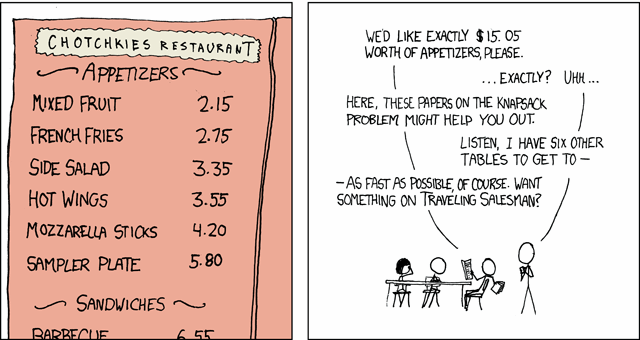
\includegraphics[width=10cm]{Figures/joke1.png}
\end{center}
\end{frame}

\begin{frame}
\begin{center}
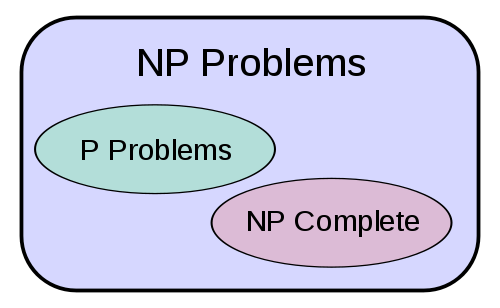
\includegraphics[width=7cm]{Figures/pnp.png}
\end{center}
\end{frame}

\begin{frame}
\begin{center}

\includegraphics[width=7cm]{Figures/joke2.png}
\end{center}
\end{frame}

\begin{frame}
Define an array of subproblems: we consider the first $i$ weights
(i.e., $[i]$) summing up to an {\em intermediate} weight limit $j$.

We define a Boolean array $R$ as follows:
$$
R(i,j)=\begin{cases}
\true & \mbox{if $\exists S\subseteq [i]$ such that $K(S) = j$} \\
\false & \mbox{otherwise}
\end{cases},
$$
for $0\leq i\leq d$ and $0\leq j\leq C$.

Once we have computed all the values of $R$ we can obtain the solution $M$ as
follows: $M=\max_{j\leq C}\{j|R(d,j)=\true\}$.
\end{frame}

\begin{frame}
Define a recurrence: we initialize $R(0,j)=\false$ for $j=1,2,\ldots,C$, and
$R(i,0)=\true$ for $i=0,1,\ldots,d$.

We now define the recurrence for computing $R$, for $i,j>0$, in a way
that hinges on whether we include object $i$ in the knapsack.

Suppose that we do {\em not} include
object $i$. Then, obviously, $R(i,j)=\true$ iff $R(i-1,j)=\true$.
\end{frame}

\begin{frame}
Suppose, on the other hand, that object $i$ {\em is} included.  Then it must
be the case that $R(i,j)=\true$ iff $R(i-1,j-w_i)=\true$ and
$j-w_i\geq 0$, i.e., there is a subset $S\subseteq[i-1]$
such that $K(S)$ is exactly
$j-w_i$ (in which case $j\geq w_i$).

\begin{center}
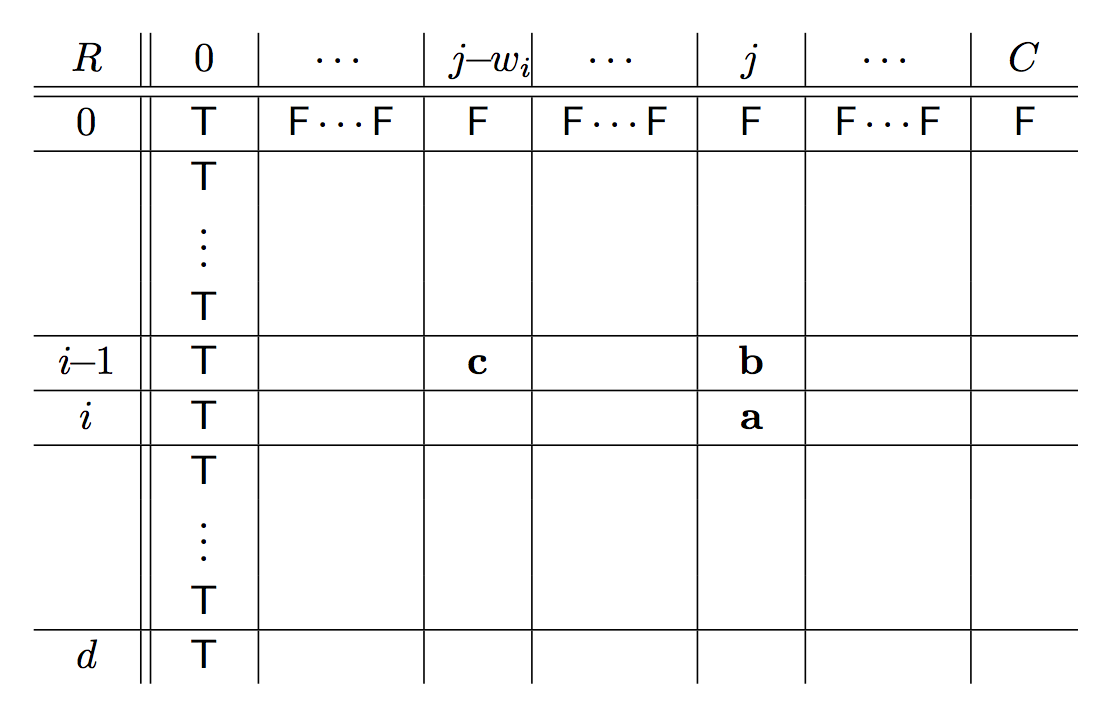
\includegraphics[width=8cm]{Figures/knp-table.png}
\end{center}
\end{frame}

\begin{frame}
Putting it all together we obtain
the following recurrence for $i,j>0$:
$$
R(i,j)=\true
\iff
R(i-1,j)=\true\vee(j\geq w_i\wedge R(i-1,j-w_i)=\true).
$$
\end{frame}

\begin{frame}
\begin{algorithmic}[1]
\STATE $S(0) \longleftarrow \true$
\FOR{$j:1..C$}
     \STATE $S(j)\longleftarrow \false$
\ENDFOR
\FOR{$i:1..d$}
     \FOR{{\bf\em decreasing} $j:C..1$}
          \IF{($j \geq w_i$ and $S(j-w_i)=\true$)}
                   \STATE $S(j) \longleftarrow \true$
          \ENDIF
     \ENDFOR
\ENDFOR
\end{algorithmic}
\end{frame}

\begin{frame}
{General Knapsack Problem}

Input: $w_1,w_2,\ldots,w_d,v_1,\ldots,v_d,C\in\mathbb{N}$ \\
Output: $\max_{S\subseteq[d]}\{V(S)|K(S)\leq C\}$,
$K(S)=\sum_{i\in S}w_i$, $V(S)=\sum_{i\in S}v_i$.

$$
V(i,j)=\max\{V(S)|S\subseteq[i]\text{ and }K(S)=j\},
$$
for $0\leq i\leq d$ and $0\leq j\leq C$.

Problem: what is the recurrence for this problem?
\end{frame}

\begin{frame}
{\bf Approximating SKS}

Greedy ``solution'' to SKS:

order the weights from heaviest to lightest, keep adding for as long as
possible.

Let $M$ be the optimal solution, and let $\bar{M}$ be the solution obtained
from the greedy approach.

Performance: $1/2$.
\end{frame}

\begin{frame}
Let $S_0$ be the set of weights we got from greedy, so $K(S_0)=\bar{M}$.

If $S_0=\emptyset$, then $\bar{M}=M$. \\
If $S_0=S$ (all weights in), then $\bar{M}=M$.

OTHERWISE:

Assume we throw out weights greater than $C$ (they won't be added anyway).
Let $w_j$ be the first weight that has been rejected, after some weights have
been added $\ldots$.
\end{frame}

\section{Activity Selection}

\begin{frame}
{\bf Activity Selection}

Input: A list of activities $(s_1,f_1,p_1),\ldots,(s_n,f_n,p_n)$,
where $p_i>0$, $s_i<f_i$ and $s_i,f_i,p_i$ are non-negative real
numbers. \\

Output:  A set $S\subseteq[n]$ of
selected activities such that no two selected activities overlap, and
the profit $P(S)= \sum_{i \in S}p_i$ is as large as possible.

An {\em activity} $i$ has a fixed start time $s_i$, finish time $f_i$
and profit $p_i$.  Given a set of activities, we want to select a
subset of non-overlapping activities with maximum total profit.
\end{frame}

\begin{frame}
Define an array of subproblems: sort the activities by their finish
times, $f_1\leq f_2\leq\ldots\leq f_n$.

As it is possible that
activities finish at the same time, we select the {\em distinct}
finish times, and denote them $u_1<u_2<\ldots<u_k$, where, clearly,
$k\le n$.

For instance, if we have activities finishing at times
1.24, 4, 3.77, 1.24, 5 and 3.77, then we partition them into four
groups: activities finishing at times $u_1=1.24$, $u_2=3.77$, $u_3=4$,
$u_4=5$.
\end{frame}

\begin{frame}
Let $u_0$ be $\min_{1\leq i\leq n}s_i$, i.e., the earliest start time.
Thus,
$$
u_0<u_1<u_2<\ldots<u_k,
$$
as it is understood that $s_i<f_i$.
Define an array $A(0..k)$ as follows:
$$
A(j)=\max_{S\subseteq[n]} \{ P(S) | \mbox{$S$ is feasible
and $f_i\leq u_j$ for each $i\in S$} \},
$$
where $S$ is {\em feasible} if no two activities in $S$ overlap.
Note that $A(k)$ is the maximum possible profit for all feasible
schedules $S$.
\end{frame}

\begin{frame}
Define a recurrence for $A(0..k)$.

In order to give such a recurrence we first define an auxiliary
array $H(1..n)$ such that $H(i)$ is the index of the largest distinct
finish time no greater than the start time of activity $i$.

Formally, $H(i)=\ell$ if $\ell$ is the largest number such that
$u_\ell \leq s_i$. To compute $H(i)$, we need to search the list of
distinct finish times.

To do it efficiently, for each $i$, apply the binary search
procedure that runs in logarithmic time in the length of the list of
distinct finish times (try $\ell=\lfloor \frac{k}{2} \rfloor $
first).

Since the length $k$ of the list of distinct finish times is
at most $n$, and we need to apply binary search for each element of
the array $H(1..n)$, the time required to compute all entries of the
array is $O(n\log n)$.
\end{frame}

\begin{frame}
We initialize $A(0)=0$,
and we want to compute $A(j)$ given that we already have
$A(0),\ldots, A(j-1)$.

Consider $u_0 < u_1 < u_2 <
\ldots < u_{j-1} < u_j $.

Can we beat profit $A(j-1)$ by scheduling some
activity that finishes at time $u_j$? Try all activities that finish
at this time and compute maximum profit in each case. We obtain the
following recurrence:
$$
A(j)=\max\{A(j-1),\max_{1\leq i\leq n}\{p_i+A(H(i))\ |\ f_i=u_j\}\},
$$
where $H(i)$ is the greatest $\ell$ such that $u_\ell\le s_i$.
\end{frame}

\begin{frame}
\begin{center}
\begin{minipage}{8cm}
\xymatrix@C=5mm{
&& \ar@{.}[ddd] & \ar@{|=|}[rrr]^a\ar@{.}[ddd]
&\ar@{.}[ddd]&\ar@{.}[ddd]& \ar@{.}[ddd] &\\
& \ar@{|=|}[rrrrr]^b\ar@{.}[dd] &&&&&& \\
&&&& \ar@{|=|}[rr]^c\ar@{.}[d] &&& \\
\ar@{<->}[rrrrrrr] &\circ&\circ&\circ&\circ&\circ&\circ& \\
 & s_b=u_{H(b)} & u_{H(a)} & s_b & s_c=u_{H(c)} & u_{j-1} & u_j &
}
\end{minipage}
\end{center}
\end{frame}

\begin{frame}
\begin{algorithmic}
\STATE $A(0)\longleftarrow 0$
\FOR{$j:1..k$}
	\STATE $\max\longleftarrow 0$
	\FOR{$i=1..n$}
		\IF{$f_i=u_j$}
			\IF{$p_i+A(H(i))>\max$}
				\STATE $\max\longleftarrow p_i+A(H(i))$
			\ENDIF
		\ENDIF
	\ENDFOR
	\IF{$A(j-1)>\max$}
		\STATE $\max\longleftarrow A(j-1)$
	\ENDIF
	\STATE $A(j)\longleftarrow\max$
\ENDFOR
\end{algorithmic}
\end{frame}

\section{Complexity}

\begin{frame}
\begin{center}
{\bf Introduction to Complexity} \\
This material is not in the IAA textbook but here: \\[5mm]

\includegraphics[width=3.5cm]{Figures/complexity.jpg}
\end{center}
\end{frame}

\begin{frame}
A TM $M$ is of \df{time complexity} $T(n)$ if whenever $M$ is given
an input $w$, $|w|=n$, then $M$ {\em halts} after making at most
$T(n)$ many moves.

\df{$L\in\text{TIME}(f(n))$} if there exists a deterministic TM $M$ of
time complexity $O(f(n))$ that decides $L$.

\df{$L\in\text{NTIME}(f(n))$} if there exists a nondeterministic TM
$M$ of time complexity $O(f(n))$ that decides $L$.

$L$ is in the class \df{P} if $L\in\text{TIME}(n^k)$ for some
fixed $k$.

$L$ is in the class \df{NP}  if $L\in\text{NTIME}(n^k)$ for some
fixed $k$.
\end{frame}

\begin{frame}
Observation: P$\subseteq$NP;  Question: NP$\subseteq$P ?

Ex.\ of a language in P:
$\{\langle G,k\rangle|\text{$G$ has a spanning tree of weight $\le k$}\}$.
($k=15$)
\begin{center}
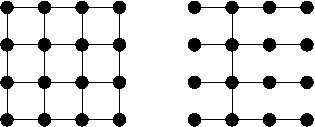
\includegraphics[width=4cm]{Figures/13.pdf}
\end{center}

Ex.\ of a language in NP believed not to be in P:
$\{\langle G,k\rangle|\text{$G$ has a complete cycle of weight $\le k$}\}$.
($k=16$)
\begin{center}
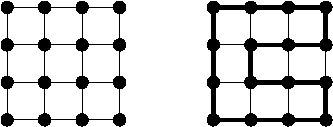
\includegraphics[width=4cm]{Figures/12.pdf}
\end{center}
\end{frame}

\begin{frame}
A graph $G$ can be encoded as an adjacency matrix.  For example, the
graph given below would have the adjacency matrix given by:

\begin{center}
\begin{minipage}{2cm}
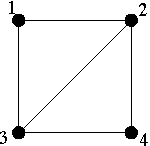
\includegraphics[width=1.4cm]{Figures/14.pdf}
\end{minipage}
\begin{minipage}{3cm}
{\footnotesize $\left[\begin{array}{cccc}
0 & 1 & 1 & 0 \\
1 & 0 & 1 & 1 \\
1 & 1 & 0 & 1 \\
0 & 1 & 1 & 0
\end{array}\right]$}
\end{minipage}
\end{center}

If $P$ is a \df{decision problem}, the related language $L_P$
consists of the encodings (under some fixed convention) of all the
``yes'' instances of $P$.

{\bf Feasibility Thesis:}
\begin{center}
Polynomial time algorithm $\equiv$ polynomial time TM.
\end{center}
\end{frame}

\begin{frame}
A problem $P_1$ is \df{reducible in polynomial time} to a
problem $P_2$ if there exists a polynomial time function $f$ such
that:
$$
\langle I\rangle\in L_{P_1}\iff
\langle f(I)\rangle\in L_{P_2}
$$

$L$ is \df{NP-complete} if:
\begin{enumerate}
\item  $L\in\text{NP}$
\item  Every language $L'\in\text{NP}$ is polynomial time reducible
to $L$.
\end{enumerate}

Ex.\ Traveling Salesman Problem

$L$ is NP-complete is {\em evidence}
of $L$ not being in P

(see {\em Computers and Intractability} by Michael Garey and David
Johnson.)
\end{frame}

\begin{frame}

{\bf Theorem:}  If $P_1$ is NP-complete, $P_2$ is in NP, and there is
a polynomial time reduction of $P_1$ to $P_2$, then $P_2$ is also
NP-complete.

{\bf Proof:} Every language $L$ in NP is reducible to
$L_{P_1}$, by completeness, and $P_1$ is reducible to $P_2$.  Enough
to show transitivity of reductions.

{\bf Theorem:}  If some NP-complete problem $P$ is in P, then P$=$NP.

{\bf Proof:}  Follows from the fact that all languages in
NP are polynomial time reducible to $P$.

%Exercises: 10.1.1--3,5--7.
\end{frame}

\begin{frame}

{\bf Satisfiability}

\df{Boolean Expressions} are built from: Boolean variables
$x,y,z,\ldots$, Boolean values $0,1$, and Boolean connectives:
$\vee,\wedge,\neg$, and parenthesis.

Ex.\ $\neg x\vee(y\wedge z)$

If $\phi$ is a Boolean expression, then a \df{truth assignment} $T$ is
an assignment of truth values to the variables of $\phi$.

Ex.\ $T(x)=0,T(y)=1,T(z)=1$, then $T(\neg x\vee(y\wedge
z))=\neg 0\vee(1\wedge 1)=1\vee 1=1$.

$T$ \df{satisfies} $\phi$ if $T(\phi)=1$,
and $\phi$ is \df{satisfiable} if $\exists T$ s.t. $T(\phi)=1$.
\end{frame}

\begin{frame}
The \df{satisfiability problem} is: given a Boolean expression,
is it satisfiable?

$\text{SAT}=\{\langle\phi\rangle|\text{$\phi$ is
satisfiable}\}$ \\ (i.e., SAT is the language corresponding to the
satisfiability problem).

{\bf Cook's Theorem:} SAT is NP-complete.

{\bf PROOF:}  SAT is in NP. \\
Let $L$ be any language in NP.  \\
We show there exists a polynomial time function $f$ s.t.:
$$
w\in L\iff f(w)=\phi\in\text{SAT}
$$
$\exists$ non-det TM $M$ s.t.\ $L=L(M)$ and $M$ always halts
within $n^k$ many steps on inputs $w$, $|w|=n$, for fixed $k$.  \\
Given $w$, $f$ outputs a Boolean formula $\phi$ which encodes a
computation of $M$ on $w$ and is satisfiable $\iff$ $M$ accepts $w$.
\end{frame}



\end{document}
